\documentclass[a4paper,10pt]{article}
\usepackage[brazilian]{babel}
\usepackage[left=2.5cm,right=2.5cm,top=3cm,bottom=2.5cm]{geometry}
\usepackage{mathtools}
\usepackage{amsthm}
\usepackage{amsmath}
%\usepackage{nccmath}
\usepackage{amssymb}
\usepackage{amsfonts}
\usepackage{physics}
%\usepackage{dsfont}
%\usepackage{mathrsfs}

\usepackage{titling}
\usepackage{indentfirst}

\usepackage{bm}
\usepackage[dvipsnames]{xcolor}
\usepackage{cancel}

\usepackage{xurl}
\usepackage[colorlinks=true]{hyperref}

\usepackage{float}
\usepackage{graphicx}
%\usepackage{tikz}
\usepackage{caption}
\usepackage{subcaption}

%%%%%%%%%%%%%%%%%%%%%%%%%%%%%%%%%%%%%%%%%%%%%%%%%%%

\newcommand{\eps}{\epsilon}
\newcommand{\vphi}{\varphi}
\newcommand{\cte}{\text{cte}}

\newcommand{\N}{\mathbb{N}}
\newcommand{\Z}{\mathbb{Z}}
\newcommand{\Q}{\mathbb{Q}}
\newcommand{\R}{\vb{R}}
\newcommand{\C}{\mathbb{C}}
\renewcommand{\S}{\hat{S}}
%\renewcommand{\H}{\s{H}}

\renewcommand{\a}{\vb{a}}
\newcommand{\nn}{\hat{n}}
\renewcommand{\d}{\dagger}
\newcommand{\up}{\uparrow}
\newcommand{\down}{\downarrow}

\newcommand{\0}{\vb{0}}
%\newcommand{\1}{\mathds{1}}
\newcommand{\E}{\vb{E}}
\newcommand{\B}{\vb{B}}
\renewcommand{\v}{\vb{v}}
\renewcommand{\r}{\vb{r}}
\renewcommand{\k}{\vb{k}}
\newcommand{\p}{\vb{p}}
\newcommand{\q}{\vb{q}}
\newcommand{\F}{\vb{F}}

\newcommand{\s}{\sigma}
%\newcommand{\prodint}[2]{\left\langle #1 , #2 \right\rangle}
\newcommand{\cc}[1]{\overline{#1}}
\newcommand{\Eval}[3]{\eval{\left( #1 \right)}_{#2}^{#3}}

\newcommand{\unit}[1]{\; \mathrm{#1}}

\newcommand{\n}{\medskip}
\newcommand{\e}{\quad \mathrm{e} \quad}
\newcommand{\ou}{\quad \mathrm{ou} \quad}
\newcommand{\virg}{\, , \;}
\newcommand{\ptodo}{\forall \,}
\renewcommand{\implies}{\; \Rightarrow \;}
%\newcommand{\eqname}[1]{\tag*{#1}} % Tag equation with name

\setlength{\droptitle}{-7em}

\theoremstyle{plain}
\newtheorem{theorem}{Teorema}[section]
%\newtheorem{defi}[theorem]{Definição}
\newtheorem{lemma}[theorem]{Lema}
%\newtheorem{corol}[theorem]{Corolário}
%\newtheorem{prop}[theorem]{Proposição}
%\newtheorem{example}{Exemplo}
%
%\newtheorem{inneraxiom}{Axioma}
%\newenvironment{axioma}[1]
%  {\renewcommand\theinneraxiom{#1}\inneraxiom}
%  {\endinneraxiom}
%
%\newtheorem{innerpostulado}{Postulado}
%\newenvironment{postulado}[1]
%  {\renewcommand\theinnerpostulado{#1}\innerpostulado}
%  {\endinnerpostulado}
%
%\newtheorem{innerexercise}{Exercício}
%\newenvironment{exercise}[1]
%  {\renewcommand\theinnerexercise{#1}\innerexercise}
%  {\endinnerexercise}
%
%\newtheorem{innerthm}{Teorema}
%\newenvironment{teorema}[1]
%  {\renewcommand\theinnerthm{#1}\innerthm}
%  {\endinnerthm}
%
\newtheorem{innerlema}{Lema}
\newenvironment{lema}[1]
  {\renewcommand\theinnerlema{#1}\innerlema}
  {\endinnerlema}
%
%\theoremstyle{remark}
%\newtheorem*{hint}{Dica}
%\newtheorem*{notation}{Notação}
%\newtheorem*{obs}{Observação}


\setlength\parindent{0pt}  % noindent in entire file

\usepackage{minted}
\usemintedstyle{vs}
\definecolor{bg}{rgb}{0.85,0.85,0.85}
\setmintedinline{bgcolor=bg}
\newcommand{\python}[1]{\mintinline{python}{#1}}
\usepackage{tcolorbox}
\tcbuselibrary{minted,skins}
\newtcblisting{Python}{
  listing engine=minted,
  colback=bg,
  colframe=black!70,
  listing only,
  minted style=vs,
  minted language=python,
  minted options={texcl=true, fontsize=\scriptsize},
  left=1mm,
}

\renewcommand{\p}{\phantom{+}}
\newcommand{\mchi}{\chi^{\Gamma^\pi_{p_z}}}
\renewcommand{\c}[1]{\textcolor{red}{#1}}

\title{\Huge{\textbf{Teoria de grupos - Exercício 3}}}
\author{Mateus Marques}

\begin{document}

\maketitle

\section*{A ligação $\pi$ da molécula de benzeno C$_6$H$_6$}

A molécula de benzeno tem geometria de um hexágono. Assim, ela possui um eixo $C_6$ (o eixo $z$), 6 eixos $C_2$ (no plano da molécula, 3 passando pelos átomos de carbono e 3 passando pelo meio das arestas do hexágono) e, além disso, ela também possui um plano de reflexão $\sigma_h$. No total, isso totaliza $12 \cdot 2 = 24$ elementos. Note que essas características correspondem unicamente ao grupo $D_{6h} = D_6 \otimes C_{1h}$.

\begin{figure}[H]
\centering
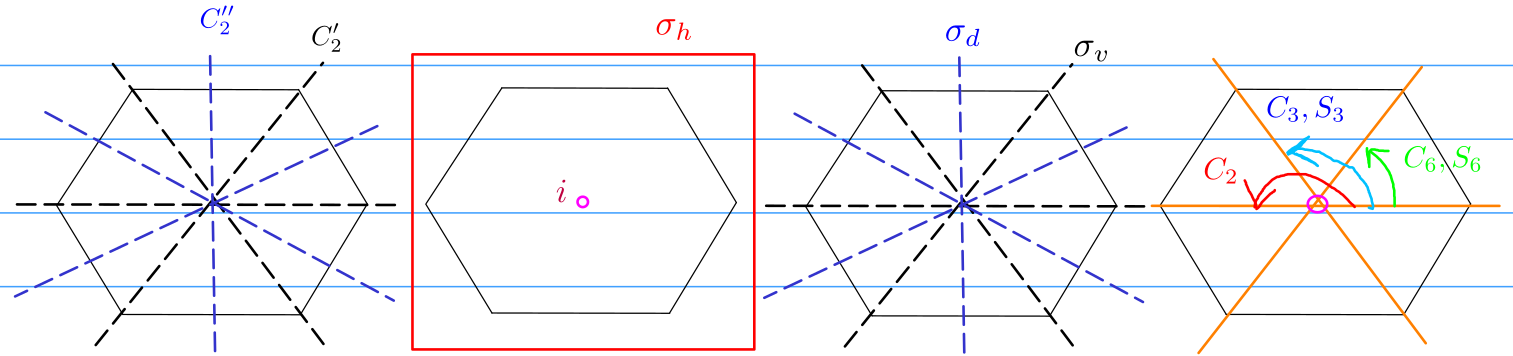
\includegraphics[width=1.0\linewidth]{fig/D6h.png}
\caption{Elementos de simetria do grupo $D_{6h}$, correspondente à molécula de benzeno C$_6$H$_6$.}
\label{fig:D6h}
\end{figure}

Agora descobriremos a representação $\Gamma^\pi_{p_z}$. Note que a base tem dimensão $6$, já que temos 6 orbitais, representados pelo vetor $(\vphi_1, \vphi_2, \vphi_3, \vphi_4, \vphi_5, \vphi_6)$. Avaliaremos os caracteres dessa representação $\Gamma^\pi_{p_z}$ para seus elementos, seguindo os desenhos da Figura \ref{fig:D6h}:
\begin{enumerate}
\item $E$ $\implies$ matriz identidade de dimensão 6, portanto $\mchi(E) = 6$.
\item $C_6$ (eixo $z$) $\implies$ troca os 6 orbitais de lugar, portanto $\mchi(C_6) = 0$.
\item $C_3$ (eixo $z$) $\implies$ troca os 6 orbitais de lugar, portanto $\mchi(C_3) = 0$.
\item $C_2$ (eixo $z$) $\implies$ troca os 6 orbitais de lugar, portanto $\mchi(C_2) = 0$.
\item $C_2'$ $\implies$ mantém 2 dos 6 orbitais inalterados e inverte a polarização, portanto $\mchi(C_2') = -2$.
\item $C_2''$ $\implies$ troca os 6 orbitais de lugar, portanto $\mchi(C_2'') = 0$.
\item $i$ $\implies$ troca os 6 orbitais de lugar, portanto $\mchi(i) = 0$.
\item $S_3$ $\implies$ troca os 6 orbitais de lugar, portanto $\mchi(S_3) = 0$.
\item $S_6$ $\implies$ troca os 6 orbitais de lugar, portanto $\mchi(S_6) = 0$.
\item $\sigma_h$ $\implies$ mantém os 6 orbitais, mas inverte a polarização de todos, portanto $\mchi(\sigma_h) = -6$.
\item $\sigma_d$ $\implies$ troca os 6 orbitais de lugar, portanto $\mchi(\sigma_d) = 0$.
\item $\sigma_v$ $\implies$ mantém 2 dos 6 orbitais e mantém a polarização, portanto $\mchi(\sigma_v) = 2$.
\end{enumerate}

Retirando a tabela de caracteres do grupo $D_{6h}$ do site \url{http://symmetry.jacobs-university.de/cgi-bin/group.cgi?group=606&option=4} e adicionando a linha com os caracteres de $\Gamma^\pi_{p_z}$, obtemos a Tabela \ref{tab:mult_D6h} abaixo.

\begin{table}[H]
\caption{Tabela de caracteres para o grupo $D_{6h}$.}
\centering

\begin{tabular} { |c|c c c c c c c c c c c c | }
\hline
$D_{6h}$ & $E$ & $2 C_6$ & $2 C_3$ & $C_2$ & $3 C_2'$ & $3 C_2''$ & $i$ & $2 S_3$ & $2 S_6$ & $\sigma_h$ & $3 \sigma_d$ & $3 \sigma_v$ \\
\hline
$A_{1g}$ & $\p1$ & $\p1$ & $\p1$ & $\p1$ & $\p1$ & $\p1$ & $\p1$ & $\p1$ & $\p1$ & $\p1$ & $\p1$ & $\p1$ \\
$A_{2g}$ & $\p1$ & $\p1$ & $\p1$ & $\p1$ & $ -1$ & $ -1$ & $\p1$ & $\p1$ & $\p1$ & $\p1$ & $ -1$ & $ -1$ \\
$B_{1g}$ & $\p1$ & $ -1$ & $\p1$ & $ -1$ & $\p1$ & $ -1$ & $\p1$ & $ -1$ & $\p1$ & $ -1$ & $\p1$ & $ -1$ \\
$\c{\boxed{B_{2g}}}$ & $\c{\p1}$ & $\c{ -1}$ & $\c{\p1}$ & $\c{ -1}$ & $\c{ -1}$ & $\c{\p1}$ & $\c{\p1}$ & $\c{ -1}$ & $\c{\p1}$ & $\c{ -1}$ & $\c{ -1}$ & $\c{\p1}$ \\
$\c{\boxed{E_{1g}}}$ & $\c{\p2}$ & $\c{\p1}$ & $\c{ -1}$ & $\c{ -2}$ & $\c{\p0}$ & $\c{\p0}$ & $\c{\p2}$ & $\c{\p1}$ & $\c{ -1}$ & $\c{ -2}$ & $\c{\p0}$ & $\c{\p0}$ \\
$E_{2g}$ & $\p2$ & $ -1$ & $ -1$ & $\p2$ & $\p0$ & $\p0$ & $\p2$ & $ -1$ & $ -1$ & $\p2$ & $\p0$ & $\p0$ \\
$A_{1u}$ & $\p1$ & $\p1$ & $\p1$ & $\p1$ & $\p1$ & $\p1$ & $ -1$ & $ -1$ & $ -1$ & $ -1$ & $ -1$ & $ -1$ \\
$\c{\boxed{A_{2u}}}$ & $\c{\p1}$ & $\c{\p1}$ & $\c{\p1}$ & $\c{\p1}$ & $\c{ -1}$ & $\c{ -1}$ & $\c{ -1}$ & $\c{ -1}$ & $\c{ -1}$ & $\c{ -1}$ & $\c{\p1}$ & $\c{\p1}$ \\
$B_{1u}$ & $\p1$ & $ -1$ & $\p1$ & $ -1$ & $\p1$ & $ -1$ & $ -1$ & $\p1$ & $ -1$ & $\p1$ & $ -1$ & $\p1$ \\
$B_{2u}$ & $\p1$ & $ -1$ & $\p1$ & $ -1$ & $ -1$ & $\p1$ & $ -1$ & $\p1$ & $ -1$ & $\p1$ & $\p1$ & $ -1$ \\
$E_{1u}$ & $\p2$ & $\p1$ & $ -1$ & $ -2$ & $\p0$ & $\p0$ & $ -2$ & $ -1$ & $\p1$ & $\p2$ & $\p0$ & $\p0$ \\
$\c{\boxed{E_{2u}}}$ & $\c{\p2}$ & $\c{ -1}$ & $\c{ -1}$ & $\c{\p2}$ & $\c{\p0}$ & $\c{\p0}$ & $\c{ -2}$ & $\c{\p1}$ & $\c{\p1}$ & $\c{ -2}$ & $\c{\p0}$ & $\c{\p0}$ \\
\hline
\hline
$\Gamma_{p_z}^\pi$ & $\p6$ & $\p0$ & $\p0$ & $\p0$ & $ -2$ & $\p0$ & $\p0$ & $\p0$ & $\p0$ & $ -6$ & $\p0$ & $\p2$ \\
\hline
\end{tabular}

\label{tab:mult_D6h}
\end{table}

Analisando ela com cuidado, vemos que a representação redutível $\Gamma^\pi_{p_z}$ se decompõe da forma
$$
\Gamma^\pi_{p_z} = B_{2g} \oplus E_{1g} \oplus A_{2u} \oplus E_{2u}.
$$

Agora basta aplicarmos os operadores de projeção para obter os orbitais simetrizados. Sendo $\Gamma$ uma das representações irredutíveis, o operador de projeção $\mathcal{P}^{(\Gamma)}$ é dado por
\begin{equation} \label{eq:projection}
\mathcal{P}^{(\Gamma)} = \frac{\ell_{\Gamma}}{h} \sum_{R \in G} \chi^{(\Gamma)}(R) P_R,
\end{equation}
onde $\ell_\Gamma$ é a dimensão da representação $\Gamma$, $h = 24$ é a ordem do grupo $G = D_{6h}$ e $P_R$ é o operador do elemento de simetria $R \in G$. Queremos utilizar a equação \ref{eq:projection} para calcular $\mathcal{P}^{(\Gamma)} \vphi_i$, para $\Gamma = B_{2g}, E_{1g}, A_{2u}, E_{2u}$. Para isso, precisaremos da ação $P_R \vphi_i$ para cada um dos 24 operadores $R \in D_{6h}$.

Como as representações irredutíveis de interesse são apenas unidimensionais ($B_{2g}$ e $A_{2u}$) ou bidimensionais ($E_{1g}$ e $E_{2u}$), basta que calculemos $P_R \vphi_1$ e $P_R \vphi_2$ para todo $R \in G$. Assim, montamos a Tabela \ref{tab:proj} com o auxílio da Figura \ref{fig:orbitais_pz} que define os orbitais $p_z$.
\begin{figure}[H]
\centering
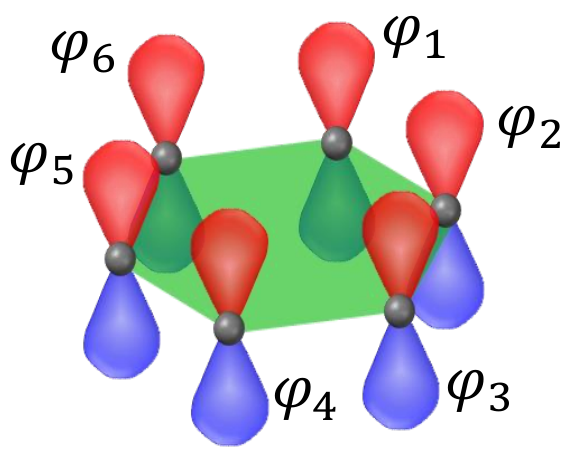
\includegraphics[width=0.6\linewidth]{fig/orbitais_pz.png}
\caption{Orbitais $p_z$ perpendiculares ao plano da molécula de benzeno C$_6$H$_6$.}
\label{fig:orbitais_pz}
\end{figure}


\begin{table}[H]
\caption{Tabela da ação dos operadores $P_R$ nos orbitais $\vphi_1, \vphi_2$.}
\centering
\footnotesize

\begin{tabular} { | c c c | }
\hline
$P_{E} \vphi_1 =  \vphi_1, P_{E} \vphi_2 =   \vphi_2$ & $P_{C_6} \vphi_1 =  \vphi_6, P_{C_6} \vphi_2 =   \vphi_1$ & $P_{C_6^5} \vphi_1 =  \vphi_2, P_{C_6^5} \vphi_2 =   \vphi_3$ \\
$P_{C_3} \vphi_1 =  \vphi_5, P_{C_3} \vphi_2 =   \vphi_6$ & $P_{C_3^2} \vphi_1 =  \vphi_3, P_{C_3^2} \vphi_2 =   \vphi_4$ & $P_{C_2} \vphi_1 =  \vphi_4, P_{C_2} \vphi_2 =   \vphi_5$ \\
$P_{C_{2,(1)}'} \vphi_1 = -\vphi_3, P_{C_{2,(1)}'} \vphi_2 = - \vphi_6$ & $P_{C_{2,(2)}'} \vphi_1 = -\vphi_5, P_{C_{2,(2)}'} \vphi_2 = - \vphi_2$ & $P_{C_{2,(3)}'} \vphi_1 = -\vphi_1, P_{C_{2,(3)}'} \vphi_2 = - \vphi_4$ \\
$P_{C_{2,(1)}''} \vphi_1 = -\vphi_2, P_{C_{2,(1)}''} \vphi_2 = - \vphi_1$ & $P_{C_{2,(2)}''} \vphi_1 = -\vphi_4, P_{C_{2,(2)}''} \vphi_2 = - \vphi_3$ & $P_{C_{2,(3)}''} \vphi_1 = -\vphi_6, P_{C_{2,(3)}''} \vphi_2 = - \vphi_5$ \\
$P_{i} \vphi_1 = -\vphi_4, P_{i} \vphi_2 = - \vphi_5$ & $P_{S_3} \vphi_1 = -\vphi_5, P_{S_3} \vphi_2 = - \vphi_6$ & $P_{S_3^2} \vphi_1 = -\vphi_3, P_{S_3^2} \vphi_2 = - \vphi_4$  \\
$P_{S_6} \vphi_1 = -\vphi_6, P_{S_6} \vphi_2 = - \vphi_1$ & $P_{S_6^5} \vphi_1 = -\vphi_2, P_{S_6^5} \vphi_2 = - \vphi_3$ & $P_{\sigma_h} \vphi_1 = -\vphi_1, P_{\sigma_h} \vphi_2 = - \vphi_2$ \\
$P_{\sigma_d^{(1)}} \vphi_1 =  \vphi_2, P_{\sigma_d^{(1)}} \vphi_2 =   \vphi_1$ & $P_{\sigma_d^{(2)}} \vphi_1 =  \vphi_4, P_{\sigma_d^{(2)}} \vphi_2 =   \vphi_3$ & $P_{\sigma_d^{(3)}} \vphi_1 =  \vphi_6, P_{\sigma_d^{(3)}} \vphi_2 =   \vphi_5$ \\
$P_{\sigma_v^{(1)}} \vphi_1 =  \vphi_1, P_{\sigma_v^{(1)}} \vphi_2 =   \vphi_2$ & $P_{\sigma_v^{(2)}} \vphi_1 =  \vphi_3, P_{\sigma_v^{(2)}} \vphi_2 =   \vphi_4$ & $P_{\sigma_v^{(3)}} \vphi_1 =  \vphi_5, P_{\sigma_v^{(3)}} \vphi_2 =   \vphi_6$ \\
\hline
\end{tabular}

\label{tab:proj}
\end{table}

Com a Tabela \ref{tab:proj} podemos realizar a soma da equação \ref{eq:projection}. Porém, além disso resultar em muitos cálculos, para as representação bidimensionais ($E_{1g}$ e $E_{2u}$) ainda teremos que ortonormalizar os orbitais. Por isso, preferi escrever um programa em \python{python} para automatizar o processo. Utilizei a biblioteca \python{sympy} para realizar os cálculos simbólicos.

\n

O código utilizado foi:

\begin{Python}
from sympy import symbols, Poly, sqrt, latex
from sympy.matrices import Matrix, GramSchmidt

f1, f2, f3, f4, f5, f6 = symbols('varphi_1 varphi_2 varphi_3 varphi_4 varphi_5 varphi_6')

h = 24  # order of the group
dim = [1, 2, 1, 2]  # the dimensions of the irreps $B_{2g}$, $E_{1g}$, $A_{2u}$, $E_{2u}$

# chi is the 4x24 matrix for the characters from the irreps [$B_{2g}$, $E_{1g}$, $A_{2u}$, $E_{2u}$] and group $D_{6h}$
#         $E$  $2 C_6$    $2 C_3$  $C_2$     $3 C_2'$      $3 C_2''$      $i$    $2 S_3$     $2 S_6$  $\sigma_h$    $3 \sigma_d$     $3 \sigma_v$
chi = [ [ 1, -1,-1,  1, 1, -1,  -1,-1,-1,  1, 1, 1,   1,  -1,-1,   1, 1, -1, -1,-1,-1, 1,1,1, ],     #  $B_{2g}$, index 0
        [ 2,  1, 1, -1,-1, -2,   0, 0, 0,  0, 0, 0,   2,   1, 1,  -1,-1, -2,  0, 0, 0, 0,0,0, ],     #  $E_{1g}$, index 1
        [ 1,  1, 1,  1, 1,  1,  -1,-1,-1, -1,-1,-1,  -1,  -1,-1,  -1,-1, -1,  1, 1, 1, 1,1,1, ],     #  $A_{2u}$, index 2
        [ 2, -1,-1, -1,-1,  2,   0, 0, 0,  0, 0, 0,  -2,   1, 1,   1, 1, -2,  0, 0, 0, 0,0,0, ], ]   #  $E_{2u}$, index 3

class Proj:     # element of symmetry from D\_6h
    def __init__(self, Pf1, Pf2):
        self.P = [Pf1, Pf2]     # action on orbitals $\varphi_1$ and $\varphi_2$

# D6h is a list with 24 elements
#              E               C6             C6\^5            C3            C3\^2             C2
D6h = [ Proj( f1,  f2), Proj( f6,  f1), Proj( f2,  f3), Proj( f5,  f6), Proj( f3,  f4), Proj( f4,  f5),
#            C2'(1)          C2'(2)         C2'(3)         C2''(1)        C2''(2)          C2''(3)
        Proj(-f3, -f6), Proj(-f5, -f2), Proj(-f1, -f4), Proj(-f2, -f1), Proj(-f4, -f3), Proj(-f6, -f5),
#              i              S3             S3\^2             S6           S6\^5            sigma\_h
        Proj(-f4, -f5), Proj(-f5, -f6), Proj(-f3, -f4), Proj(-f6, -f1), Proj(-f2, -f3), Proj(-f1, -f2),
#           sigma\_d(1)     sigma\_d(2)      sigma\_d(3)     sigma\_v(1)      sigma\_v(2)     sigma\_v(3)
        Proj( f2,  f1), Proj( f4,  f3), Proj( f6,  f5), Proj( f1,  f2), Proj( f3,  f4), Proj( f5,  f6),  ]

# irrep is the index 0, 1, 2, 3 for $B_{2g}$, $E_{1g}$, $A_{2u}$, $E_{2u}$
# phi is the index 0, 1 for $\varphi_1$ or $\varphi_2$
def proj_irrep(irrep, phi):
    soma = 0
    for R in range(len(D6h)):
        soma += chi[irrep][R] * D6h[R].P[phi]   # soma da equação (1)
    return soma * dim[irrep] / h

def norm(u):  # norma de um vetor
    soma = 0
    for e in u:
        soma += e**2
    return sqrt(soma)

def normalize(L):   # normaliza um vetor, especificado pela lista L
    norma = norm(L)
    for i in range(len(L)):
        L[i] /= norma

def myappend(psis, proj):   # macro para montar a lista de vetores
    psi = Poly(proj).coeffs()
    normalize(psi)
    psis.append(Matrix(psi))

def get_var(coeffs, vars):  # colocar em formato de variável simbólica do sympy
    var = 0
    for i in range(len(coeffs)):
        var += coeffs[i] * vars[i]
    return var
\end{Python}

\begin{Python}
def main():
    vars = [f1, f2, f3, f4, f5, f6]
    psis = []
    myappend(psis, proj_irrep(0, 0))    # $\mathcal{P}^{(B_{2g})} \varphi_1$
    myappend(psis, proj_irrep(1, 0))    # $\mathcal{P}^{(E_{1g})} \varphi_1$
    myappend(psis, proj_irrep(1, 1))    # $\mathcal{P}^{(E_{1g})} \varphi_2$
    myappend(psis, proj_irrep(2, 0))    # $\mathcal{P}^{(A_{2u})} \varphi_1$
    myappend(psis, proj_irrep(3, 0))    # $\mathcal{P}^{(E_{2u})} \varphi_1$
    myappend(psis, proj_irrep(3, 1))    # $\mathcal{P}^{(E_{2u})} \varphi_2$

    print("B2g")
    print("$$")
    print(latex(get_var(psis[0], vars)))  # $\mathcal{P}^{(B_{2g})} \varphi_1$
    print("$$")
    print()

    print("E1g")
    out_E1g = GramSchmidt(psis[1:3], orthonormal=True)  # ortonormalização por Gram-Schmidt em $E_{1g}$
    print("$$")
    print(latex(get_var(out_E1g[0], vars)))  # $\mathcal{P}^{(E_{1g})} \varphi_1$
    print("$$")
    print("$$")
    print(latex(get_var(out_E1g[1], vars)))  # $\mathcal{P}^{(E_{1g})} \varphi_2$
    print("$$")
    print()

    print("A2u")
    print("$$")
    print(latex(get_var(psis[3], vars)))  # $\mathcal{P}^{(B_{2g})} \varphi_1$
    print("$$")
    print()

    print("E2u")
    out_E2u = GramSchmidt(psis[4:6], orthonormal=True)  # ortonormalização por Gram-Schmidt em $E_{2u}$
    print("$$")
    print(latex(get_var(out_E2u[0], vars)))  # $\mathcal{P}^{(E_{2u})} \varphi_1$
    print("$$")
    print("$$")
    print(latex(get_var(out_E2u[1], vars)))  # $\mathcal{P}^{(E_{2u})} \varphi_2$
    print("$$")

if __name__ == '__main__':
    main()
\end{Python}

Note que eu utilizei a função \python{sympy.matrices.GramSchmidt} para ortonormalizar os orbitais das representações bidimensionais ($E_{1g}$ e $E_{2u}$).

\n

O código printa os orbitais diretamente em formato \LaTeX. Do output dele eu só deixei os fatores em evidência para simplificar. Obtive:

\begin{itemize}
\item $B_{2g}$:
$$
\psi_{B_{2g}} =
\frac{1}{\sqrt{6}} (\varphi_{1} - \varphi_{2} + \varphi_{3} - \varphi_{4} + \varphi_{5} - \varphi_{6})
$$

\item $E_{1g}$ (bidegenerado):
$$
\psi_{E_{1g}}^{(1)} =
\frac{1}{2\sqrt{3}} (
2 \varphi_{1} + \varphi_{2} - \varphi_{3} - 2 \varphi_{4} - \varphi_{5} + \varphi_{6}
)
$$
$$
\psi_{E_{1g}}^{(2)} =
\frac{1}{2} (
\varphi_{2} + \varphi_{3} - \varphi_{5} - \varphi_{6}
)
$$

\item $A_{2u}$:
$$
\psi_{A_{2u}} =
\frac{1}{\sqrt{6}} (
\varphi_1 + \varphi_2 + \varphi_3 + \varphi_4 + \varphi_5 + \varphi_6
)
$$

\item $E_{2u}$ (bidegenerado):
$$
\psi_{E_{2u}}^{(1)} =
\frac{1}{2\sqrt{3}} (
2 \varphi_{1} - \varphi_{2} - \varphi_{3} + 2 \varphi_{4} - \varphi_{5} - \varphi_{6}
)
$$
$$
\psi_{E_{2u}}^{(2)} =
\frac{1}{2} (
\varphi_{2} - \varphi_{3} + \varphi_{5} - \varphi_{6}
)
$$
\end{itemize}

\end{document}
